\section{Обработка результатов измерений}
\subsection{Определение $T_2$}
Для времени поперечной релаксации после подачи импульсов \textit{CPMG} мы ожидаем зависимость:
\begin{equation}
\label{eq:M2-from-T2}
M (2n \tau) = M_0 \exp \left( -\dfrac{2n\tau}{T_2} \right)
\end{equation}
Спектометр подавал импульсы с разными $ \tau $.
\subsubsection{Раствор соли $MnSO_4$}
Исходные экспериментальные данные хорошо похожи на экспоненту (график \ref{fig:mnt2exper})
\begin{figure}[H]
	\hspace{-1em}
	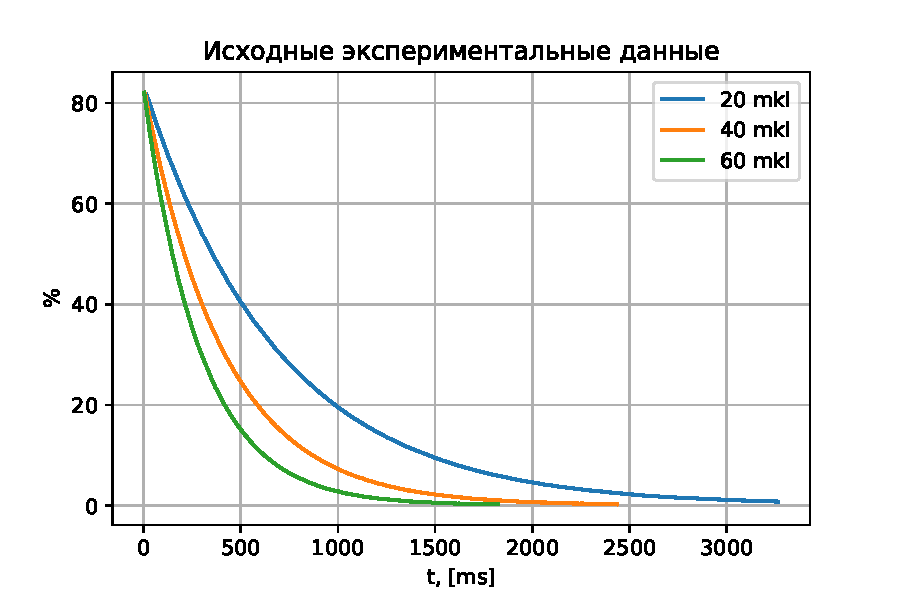
\includegraphics[width=1.0\linewidth]{data/Mn_T_2_exper}
	\caption{Экспериментальные данные в опыте по определению $ T_2 $ для соли $ Mn SO_4 $}
	\label{fig:mnt2exper}
\end{figure}

Для определения $ T_2 $ построим график $ \ln \left(\dfrac{M}{M_0} \right) = f(\tau) $. Ожидается линейная зависимость с наклоном $ k = -1/T_2 $ (график \ref{fig:mnt2reg}).

\begin{figure}[!h]
%	\centering
	\hspace{-1em}
	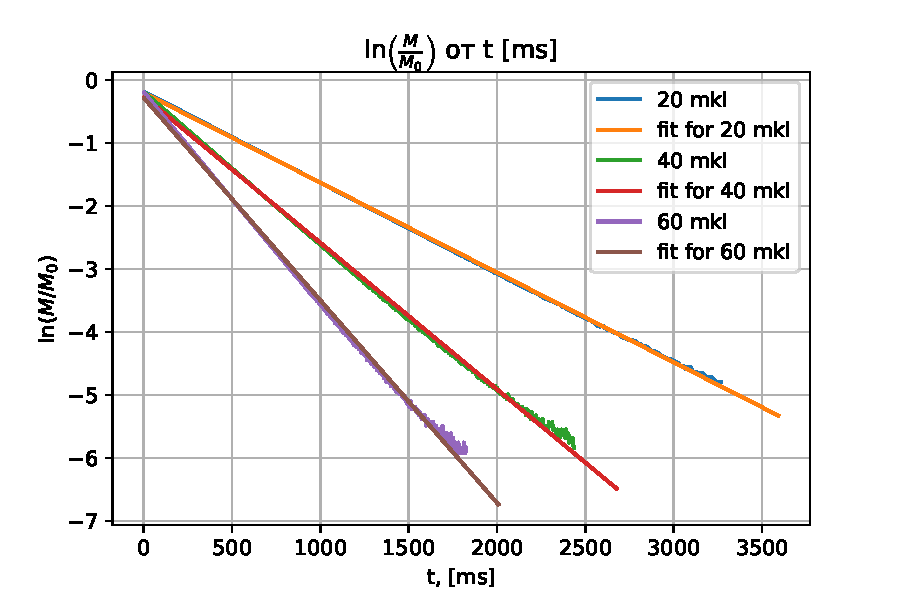
\includegraphics[width=1.0\linewidth]{data/Mn_T_2_reg}
	\caption{Линеаризация в опыте по определению $ T_2 $ для соли $ Mn SO_4 $}
	\label{fig:mnt2reg}
\end{figure}

Мы находим $ T_2 $ для различных концентраций (см. таблицу \ref{table:all-T})
\newpage

\subsubsection{Раствор $Na_2 SO_4$}
Производим аналогичные подсчеты и строим те же графики (графики \ref{fig:nat2exper} и \ref{fig:nat2reg}).

\begin{figure}[h]
	\hspace{-1em}
	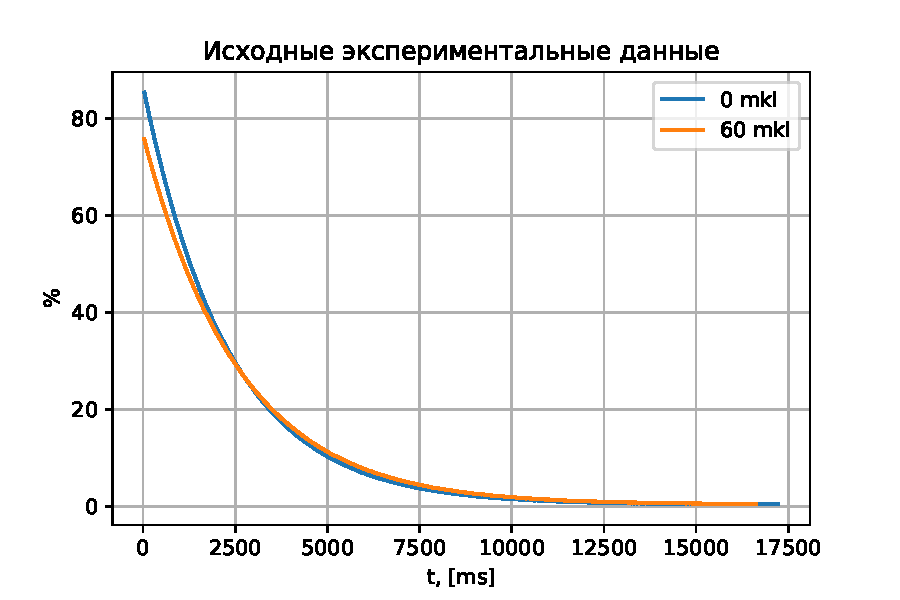
\includegraphics[width=1.0\linewidth]{data/Na_T_2_exper}
	\caption{Экспериментальные данные в опыте по определению $ T_2 $ для соли $ Na_2 SO_4 $}
	\label{fig:nat2exper}
\end{figure}
\begin{figure}[H]
	\hspace{-1em}
	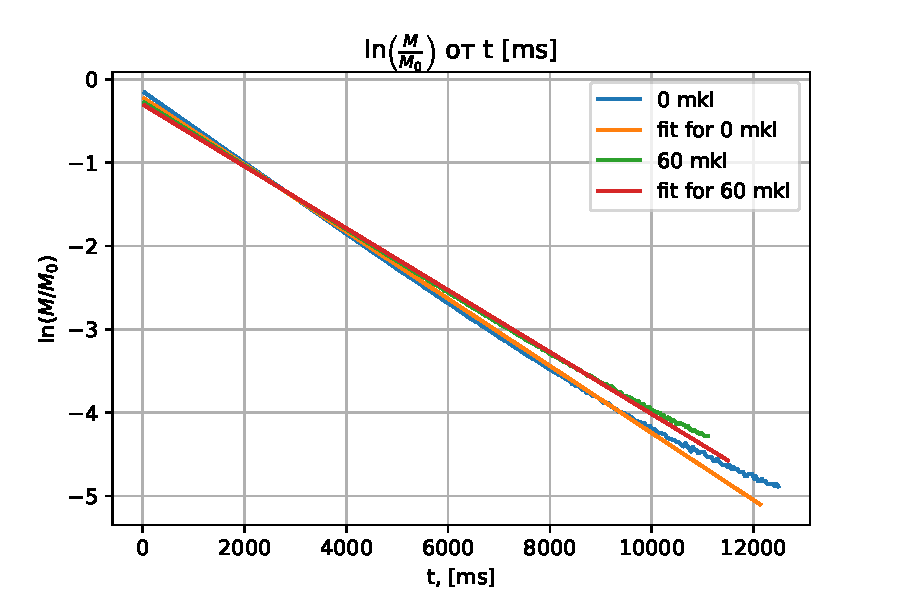
\includegraphics[width=1.0\linewidth]{data/Na_T_2_reg}
	\caption{Линеаризация в опыте по определению $ T_2 $ для соли $ Na_2 SO_4 $}
	\label{fig:nat2reg}
\end{figure}

\subsection{Определение $ T_1 $}
Для определения $ T_1 $ использовалось приложение <<\textit{t1\_saturation\_recovery.app}>>, задающее импульсную последовательность насыщение-восстановление. Ожидается теоретическая зависимость:

\begin{equation}
\label{eq:M_parall-from-T1}
M_{||} (\tau_1) = M_0 \left(1 - \exp \left( -\dfrac{\tau_1}{T_1} \right) \right)
\end{equation}

\subsubsection{Раствор $ Mn SO_4 $}
Посмотрим на экспериментальные точки (график \ref{fig:mnt1exp}). Это экспоненциальный процесс, приходящий к насыщению (как и предсказывает теория):

\begin{figure}[!h]
	\hspace{-1em}
	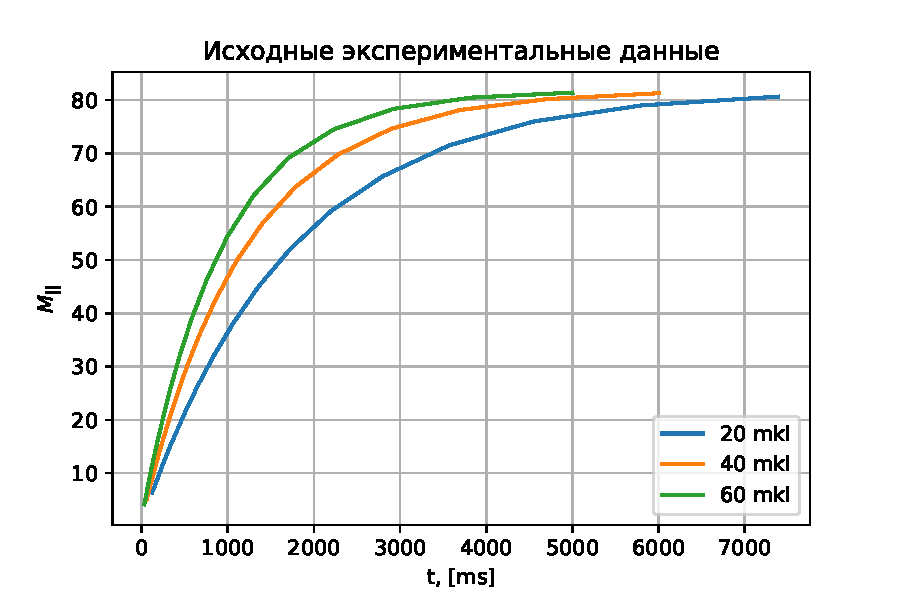
\includegraphics[width=1.0\linewidth]{data/Mn_T_1_exp}
	\caption{Экспериментальные данные в опыте по определению $ T_1 $ для соли $ Mn SO_4 $}
	\label{fig:mnt1exp}
\end{figure}

Построим график $ \ln \left( 1 - \dfrac{M_{||} (\tau_1)}{M_0} \right) = f(\tau_1)$. Ожидаем линейную зависимость с угловым коэффициентом $ k = -1/T_1 $ (график \ref{fig:mnt1reg}):

\begin{figure}[h]
	\hspace{-1em}
	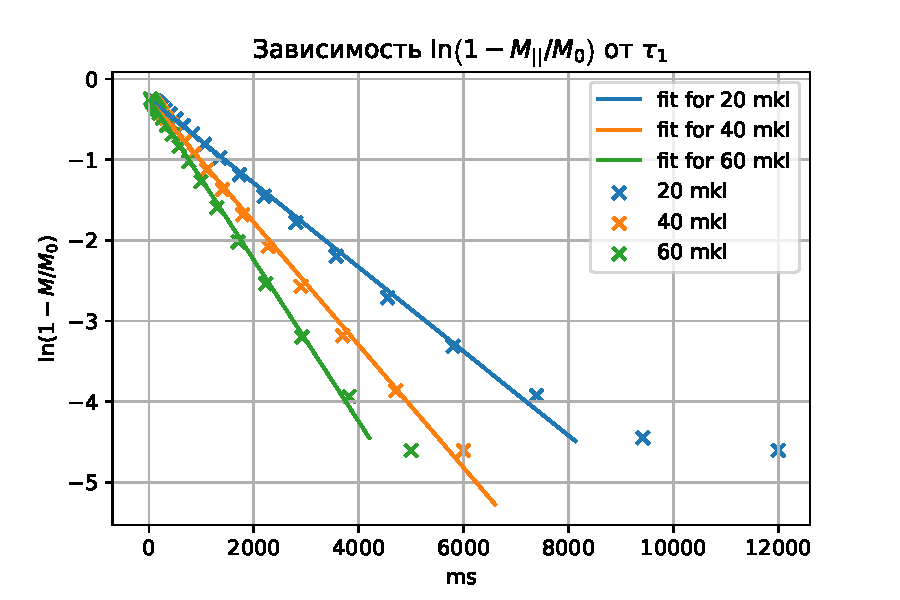
\includegraphics[width=1.0\linewidth]{data/Mn_T_1_reg}
	\caption{Линеаризация в опыте по определению $ T_1 $ для соли $ Mn SO_4 $}
	\label{fig:mnt1reg}
\end{figure}

Полученные $ T_1 $ из регрессии занесем в таблицу \ref{table:all-T}.

\newpage
\subsubsection{Раствор $Na_2 SO_4$}
Приведем аналогичные графики для растворов $ Na_2 SO_4 $ различной концентрации. Экспериментальные данные представлены на графике \ref{fig:nat1exp}.

Линеаризация экспериментальных данных приведена на графике \ref{fig:nat1reg}.

Полученные из линейной регрессии $ T_1 $ занесены в таблицу \ref{table:all-T}.
\newpage

\begin{figure}[h]
	\hspace{-1em}
	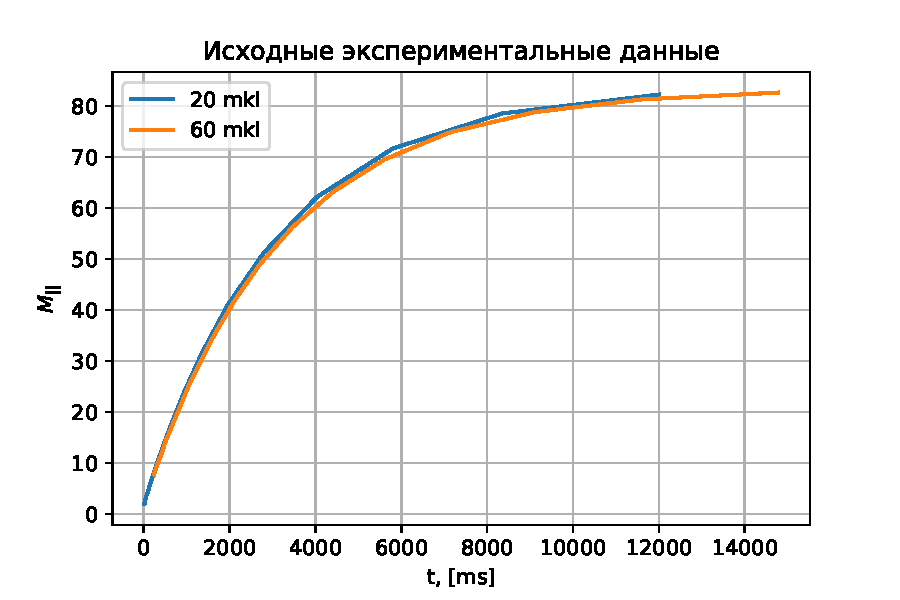
\includegraphics[width=1.0\linewidth]{data/Na_T_1_exp}
	\caption{Экспериментальные данные в опыте по определению $ T_1 $ для соли $ Na_2 SO_4 $}
	\label{fig:nat1exp}
	\vspace{-2em}
\end{figure}
\begin{figure}[H]
	\hspace{-1em}
	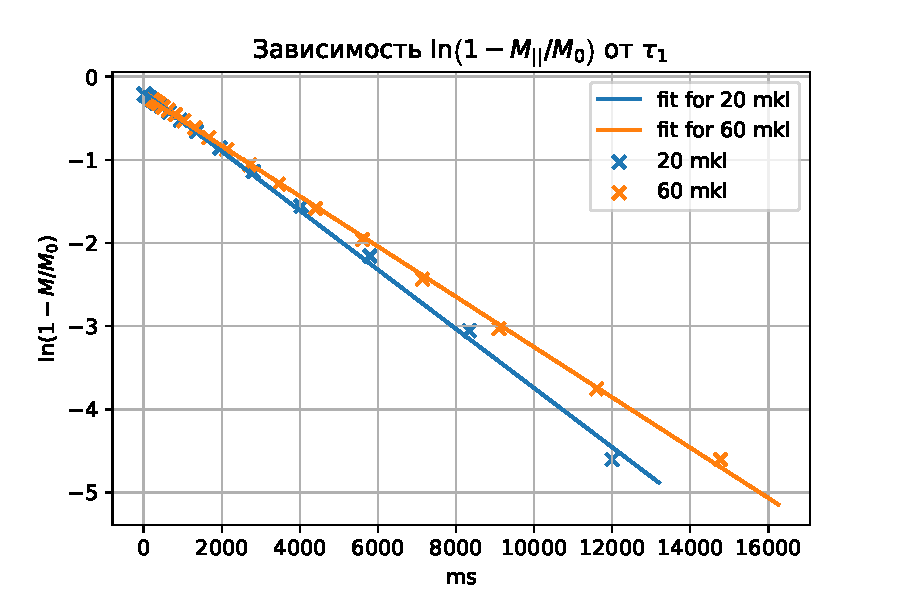
\includegraphics[width=1.0\linewidth]{data/Na_T_1_reg}
	\caption{Линеаризация в опыте по определению $ T_1 $ для соли $ Na_2 SO_4 $}
	\label{fig:nat1reg}
\end{figure}

\subsection{Определение $ T_2^* $}
Регистрация $ T_2^* $ осуществляется в приложении <<\textit{fid.app}>> по скорости спада свободной индукции (скорость спада определяется значением $ 1/T_2^* $). Приведем экспериментальную зависимость спада для $ Mn SO_4 $ (график \ref{fig:mnfid}) и $ Na_2 SO_4 $ (график \ref{fig:nafid}). В случае $ Na_2 SO_4 $ проведено дополнительное измерение для чистой воды.

\begin{figure}[h]
	\hspace{-1em}
	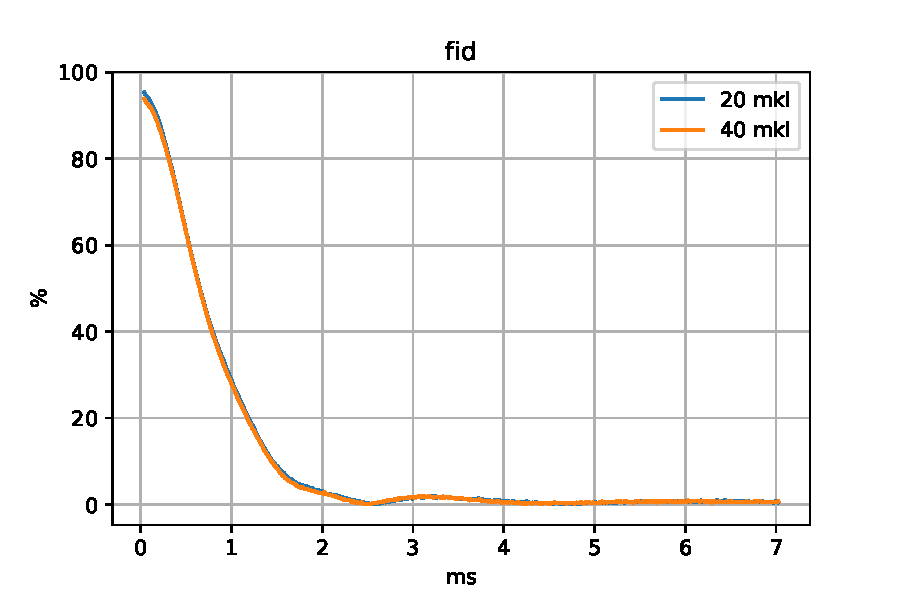
\includegraphics[width=1.0\linewidth]{data/Mn_fid}
	\caption{Регистрация $ T_2^* $ для $ Mn SO_4 $}
	\label{fig:mnfid}
\end{figure}

\begin{figure}[h]
	\hspace{-1em}
	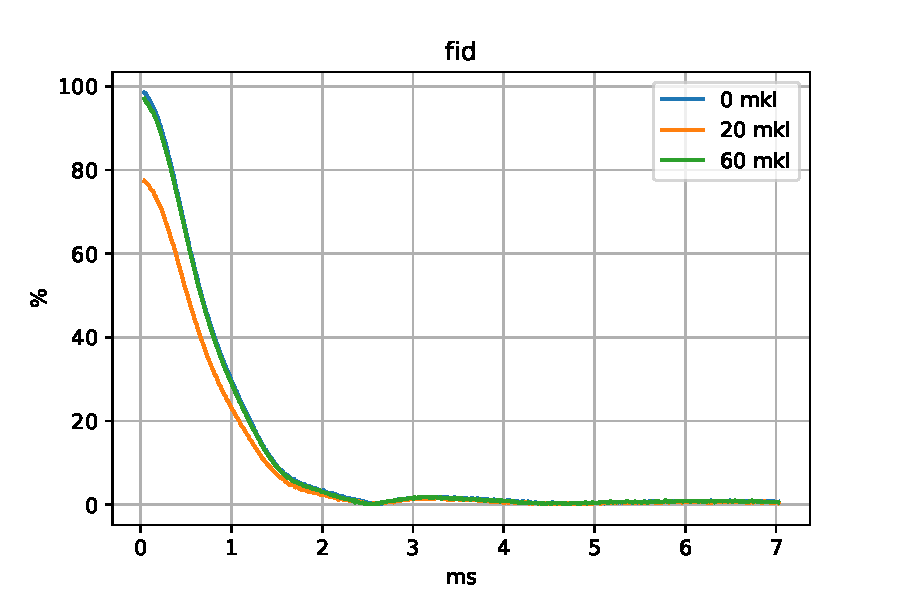
\includegraphics[width=1.0\linewidth]{data/Na_fid}
	\caption{Регистрация $ T_2^* $ для $ Na_2 SO_4 $}
	\label{fig:nafid}
\end{figure}

По времени спада в два раза можно определить $ T_2^* $ (было выполнено программой в автоматическом режиме). Эти данные занесены в таблицу \ref{table:all-T}.



\begin{table}[ht]
	\caption{Сводная таблица с результатами}
	\label{table:all-T}
	\centering
	\begin{tabular}{|l|c|r|r|r|r|}
		\toprule
		Соль &     $V$, мкл &          $T_1$ &          $T_2$ &  $T_2^*$ \\
		\midrule
		$MnSO_4$  	&  20 &  1916.731102 &   700.953789 &  0.68 \\
		$MnSO_4$  	&  40 &  1314.994472 &   429.785639 &  0.68 \\
		$MnSO_4$ 	&  60 &   997.851468 &   310.944742 &  0.68 \\
		$Na_2 SO_4$ &   0 &          --	 &  2563.068945 &  0.68 \\
		$Na_2 SO_4$ &  20 &  2810.293796 &          --  &  0.68 \\
		$Na_2 SO_4$ &  60 &  3305.489338 &  2714.577389 &  0.68 \\
		\bottomrule
	\end{tabular}
\end{table}
